% Straight up stealing preamble from Eli Holmes 
%%%%%%%%%%%%%%%%%%%%%%%%%%%%%%%%%%%%%%START PREAMBLE THAT IS THE SAME FOR ALL EXAMPLES
\documentclass{article}

%Required: You must have these
\usepackage{Sweave}
\usepackage{graphicx}
\usepackage{tabularx}
\usepackage{hyperref}
\usepackage{natbib}
\usepackage{pdflscape}
\usepackage{array}
\usepackage{gensymb}
\usepackage{authblk}
\renewcommand{\baselinestretch}{1.8}
%\usepackage{lineno}
%\usepackage[backend=bibtex]{biblatex}
%Strongly recommended
 %put your figures in one place
 
%you'll want these for pretty captioning
\usepackage[small]{caption}

\setkeys{Gin}{width=0.8\textwidth} %make the figs 50 perc textwidth
\setlength{\captionmargin}{30pt}
\setlength{\abovecaptionskip}{0pt}
\setlength{\belowcaptionskip}{10pt}
% manual for caption http://www.dd.chalmers.se/latex/Docs/PDF/caption.pdf

%Optional: I like to muck with my margins and spacing in ways that LaTeX frowns on
%Here's how to do that
 \topmargin -2cm 
 \oddsidemargin -0.04cm 
 \evensidemargin -0.04cm % same as oddsidemargin but for left-hand pages
 \textwidth 16.59cm
 \textheight 22.94cm 
 %\pagestyle{empty} % Uncomment if don't want page numbers
 %\parskip 7.2pt  % sets spacing between paragraphs
 %\renewcommand{\baselinestretch}{1.5} 	% Uncomment for 1.5 spacing between lines
\parindent 0pt% sets leading space for paragraphs
\usepackage[doublespacing]{setspace}
%\doublespacing

%Optional: I like fancy headers
\usepackage{fancyhdr}
\pagestyle{fancy}
\fancyhead[LO]{Soil moisture and plant phenology}
\fancyhead[RO]{2018}

%%%%%%%%%%%%%%%%%%%%%%%%%%%%%%%%%%%%%%END PREAMBLE THAT IS THE SAME FOR ALL EXAMPLES

%Start of the document
\begin{document}

% \SweaveOpts{concordance=TRUE}
\bibliographystyle{/Users/aileneettinger/citations/Bibtex/styles/ecol_let.bst}

\title{Soil moisture interacts with temperature to affect plant phenology}
\begin{singlespace}

\author[1,2,a]{A.K. Ettinger}
\author[3,b]{J.S. Dukes}
\author[4,c]{M.R. Johnston}
\author[5,d]{C.R. Rollinson}
\author[1,4,6,e]{E.M. Wolkovich}

\affil[1]{Arnold Arboretum of Harvard University, Boston, Massachusetts 02131, USA}

\affil[2]{Tufts University, Medford, Massachusetts 02155, USA}


\affil[3]{Department of Forestry \& Natural Resources and Department of Biological Sciences, Purdue University, West Lafayette, Indiana 47907, USA}

\affil[4]{Department of Organismic \& Evolutionary Biology, Harvard University, Cambridge, Massachusetts 02138, USA}

\affil[5]{The Morton Arboretum, Lisle, Illinois 60532, USA}

\affil[6]{Forest \& Conservation Sciences, Faculty of Forestry, University of British Columbia, Vancouver, BC, Canada}

\affil[a]{Corresponding author; email: aettinger@fas.harvard.edu; phone: 781-296-4821; mailing address: 1300 Centre Street, Boston, Massachusetts 02140, USA }

%\affil[d]{jsdukes@purdue.edu}

%\affil[f]{mjohnston@g.harvard.edu}

%\affil[h]{crollinson@mortonarb.org}

%\affil[j]{e.wolkovich@ubc.ca}

\date{\today}
\maketitle %put the fancy title on
%\tableofcontents %add a table of contents

%\textbf{Statement of authorship} 
%All authors conceived of this manuscript, which began at a Radcliffe Exploratory Seminar in 2016, and all authors contributed to manuscript revisions. AKE and EMW conceived of the idea for the literature review, database compilation, and related Radcliffe Exploratory Seminar. AKE compiled the datasets; AKE analyzed the data and created the figures; AKE wrote the manuscript.

%\textbf{Data Accessibility} %Data accessibility statement: The statement must confirm that, should the manuscript be accepted, the data supporting the results will be archived in an appropriate public repository such as Dryad or Figshare and the data DOI will be included at the end of the article.
%The MC3E and ExPhen databases are available at KNB \citep{ettinger2018}, along with all R code from the analyses included in this paper. (Currently, metadata are published there; the full databases and R code are available to reviewers on github.) 

%\textbf{Running title} 
%\textbf{Key words} global warming, warming experiment, microclimate, phenology, direct and indirect effects, active-warming, target temperature
\end{singlespace}


\clearpage
%%%%%%%%%%%%%%%%%%%%%%%%%%%%%%%%%%%%%%%%%%%%%%%%%%%
%\linenumbers
\section*{Abstract}

\section* {Introduction}
\begin{singlespace}
\begin{enumerate}
\item Phenology has shifted earlier with climate change. These shifts, which have occurred around the world, are generally attributed to warming temperature, since temperature is a well-studied driver of phenology.  Chilling, forcing. 
\item In addition to warmer temperatures, climate change is expected to alter precipitation patterns. Some places may get wetter, others may get drier. The ways that changes in precipitation will affect phenology has recieved less attention. 
\item Tree water status can affect phenology, particularly in dry, tropical forests. Budburst,flowering and leaf drop phenology have also been related to tree water status in dry ecosystems \citep{essiamah1986,reich1984, van1993}. 
\item Physiology and mechanisms for soil moisture to affect phenology. Budburst can be slowed by water stress through inhibiting cell elongation \citep{essiamah1986}.
\item Climate change experiments offer a valuable tool to study climate change impacts on phenology, especially because they often manipulate precipitation, in addition to temperature, have been used to understand how global warming may affect phenology. Previous analysis of phenology in climate change experiments have generally focused on effects of warming. 
\item Do we need to discuss discrepencies between observations and experiments?

\item Here we use two databases of experimental climate change and phenology data to understand how soil moisture affects plant phenology. We also compare phenological sensitivity to temperature and soil moisture in experiments to sensitivity in observational studies. 
\end{enumerate}
 \underline{We ask three specific questions:}
\begin{enumerate}
\item{How do climate manipulations (target warming, precipitation manipulations) affect soil moisture?}
\item{How does soil moisture interact with temperature to affect phenology?}
\item{Does warming affect soil moisture similarly in experimental and non-experimental data?}
\end{enumerate}
\end{singlespace}

\section* {Methods}
\begin{singlespace}
\underline{Data}: Experimental data from MC3E and ExPhen databases, observational data from Duke (soil moisture, temp data) and Harvard Forest (soil moisture and O'Keefe phenology data). 
\underline{Analysis}:
\begin{enumerate}
\item How do climate manipulations affect soil moisture and temperature?
\begin{enumerate}
\item Fit a multilevel model: response variable is soil moisture (from experiments in MC3E database), explanatory variables are temperature, precipitation, and their interaction. Random slopes and intercepts for site; random intercepts only for doy nested within year. We the following equations to understand effects of experimental temperature (\textit{eT}) and experimental preciptation (\textit{eP}) treatments on soil moisture . 

\begin{equation}
y_{i}=\alpha_{site[year[doy[i]]]}+ \beta_{1 site[i]}eT_i+\beta_{2 site[i]}eP_i+\beta_{3 site[i]}eT_ieP_i+\epsilon_{i}
\end{equation}
\begin{equation}
\alpha_{site[year[doy]]}\sim N(\mu_{site[year]}, \sigma_{site[year]})
\end{equation}

\begin{equation}
\mu_{site[year]} \sim N(\mu_{sy}, \sigma_{sy})
\end{equation}

\begin{equation}
\mu_{sy} \sim N(\mu_{s}, \sigma_{s})
\end{equation}

\begin{equation}
\beta_{1 site} \sim N(\mu_{\beta1}, \sigma_{\beta1})
\end{equation}

\begin{equation}
\beta_{2 site} \sim N(\mu_{\beta2}, \sigma_{\beta2})
\end{equation}

\begin{equation}
\beta_{3 site} \sim N(\mu_{\beta3}, \sigma_{\beta3})
\end{equation}
\end{enumerate}

\item How does soil moisture affect phenology?
\begin{enumerate}
\item Fit models with soil moisture (SM), temperature (T), and interaction to phenology response data (budburst, leafout, flowering, fruiting, senesence). Data are from experiments (MC3E and ExPhen). Note: excluding conifers for now.
\item{\textbf{Equations}: Response variable (\textit{y}) is day of year of the phenological event. PRedictors are measured air temperature (\textit{T}) and soil moisture(\textit{SM}). Random effects are species (random slopes and intercepts); site and for year nested within site (random intercepts).}

\begin{equation}
y_{i}=\alpha_{sp[i],site[year[i]]}+ \beta_{1 sp[i]}T_i+\beta_{2 sp[i]}SM_i+\beta_{3 site[i]}T_iSM_i+\epsilon_{i}
\end{equation}
\begin{equation}
\alpha_{sp}\sim N(\mu_{sp}, \sigma_{sp})
\end{equation}

\begin{equation}
\mu_{site[year]} \sim N(\mu_{sy}, \sigma_{sy})
\end{equation}

\begin{equation}
\mu_{sy} \sim N(\mu_{s}, \sigma_{s})
\end{equation}

\begin{equation}
\beta_{1 sp} \sim N(\mu_{\beta1}, \sigma_{\beta1})
\end{equation}

\begin{equation}
\beta_{2 sp} \sim N(\mu_{\beta2}, \sigma_{\beta2})
\end{equation}

\begin{equation}
\beta_{3 sp} \sim N(\mu_{\beta3}, \sigma_{\beta3})
\end{equation}
\end{enumerate}

\item Does warming affect soil moisture and phenology similarly in experimental and non-experimental data?

\begin{enumerate}
\item Think on best model and how to model soil moisture as a function of temperature (\textit{T}, annual? seasonal?) and precipitation (\textit{P}, annual? seasonal?). For now, \textit{y} is daily moisture across multiple years and \textit{T} is MAT and \textit{P} is percent different than mean over available time series. We use this approach to make the observational data comparable to experimental data in Question 1 above.
\begin{equation}
y_{i}=\alpha_{doy[i]}+\beta_{1 site[i]}T_i+\beta_{2 site[i]}P_i+\beta_{3 site[i]}T_iP_i+\epsilon_{i}
\end{equation}

\begin{equation}
\alpha_{doy} \sim N(\mu_{doy}, \sigma_{doy})
\end{equation}

\begin{equation}
\alpha_{site[year]} \sim N(\mu_{sy}, \sigma_{sy})
\end{equation}

\begin{equation}
\mu_{sy} \sim N(\mu_{s}, \sigma_{s})
\end{equation}
\begin{equation}
\alpha_{sp} \sim N(\mu_{sp}, \sigma_{sp})
\end{equation}

\item We can compare \ensuremath{\beta_{1}},\ensuremath{\beta_{2}}, and \ensuremath{\beta_{3}} in experiments and observations. 

\end{enumerate}
\end{enumerate}
\end{singlespace}

\section* {Results}
\begin{singlespace}

\begin{enumerate}
\item {\textbf{How do climate manipulations affect soil moisture and temperature?}}
\begin{enumerate}
\item{12 sites included: exps 1-5, 7-9,10 and 12-14}
\item{Target temp has a negative effect on soil moisture. (Figure \ref {fig:soilmois})}
\item{Precip treatment has a positive effect on soil moisture.(Figure \ref {fig:soilmois})}
\item{Effects vary by site. (One site, exp07, has positive effect of temperature).}
\item \underline{For supplement}: Fit different models for different seasonal temperatures used in Question 2 (phenology models).
\end{enumerate}

\item{\textbf{How does soil moisture affect phenology?
}}
\begin{enumerate}
\item{Air temperature (seasonal) has a negative effect on phenology for all phenophases except senescence, which has a positive effect (Figure \ref{fig:bb}). Magnitude varies among sites and species.}
\item{Moisture has a negative effect on phenology for all phenophases. Magnitude varies among sites and species. }
\item \underline{For supplement}: Figures of fruiting and senescence (fewer sites)
\end{enumerate}
\item {\textbf{Does warming affect soil moisture and phenology similarly in experimental and non-experimental data?}}
\end{enumerate}
\end{singlespace}

\section* {Discussion}

\section* {Conclusions}

\bibliography{/Users/aileneettinger/citations/Bibtex/mylibrary}

\clearpage
\section* {Figures}
\clearpage
 \begin{figure}[h]
\centering
 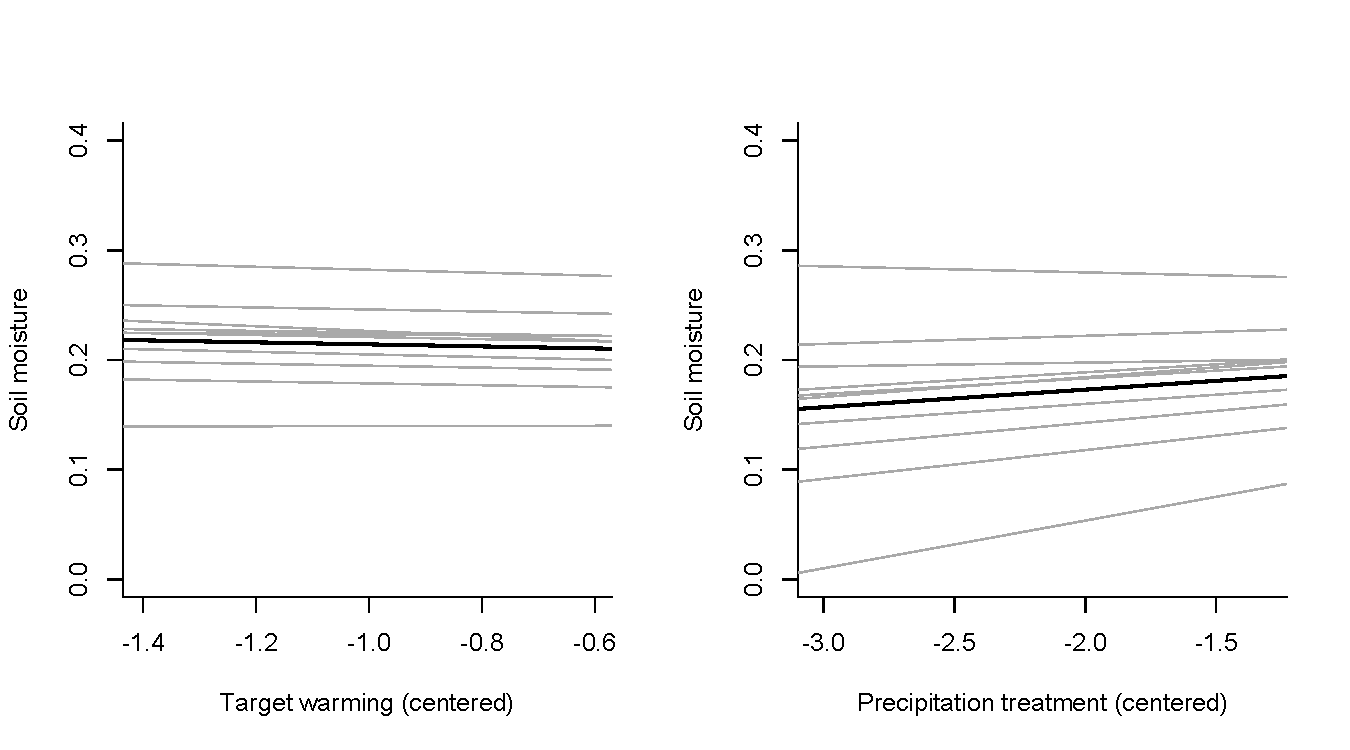
\includegraphics{/Users/aileneettinger/git/radcliffe/Analyses/soilmoisture/figures/smvstargtemp_smvspreciptreat_lines.pdf}
 \caption{\textbf{Effects of target temperature and precipitation treatments on soil moisture.}} 
 \label{fig:soilmois}
 \end{figure}

\begin{figure}[h]
\centering
 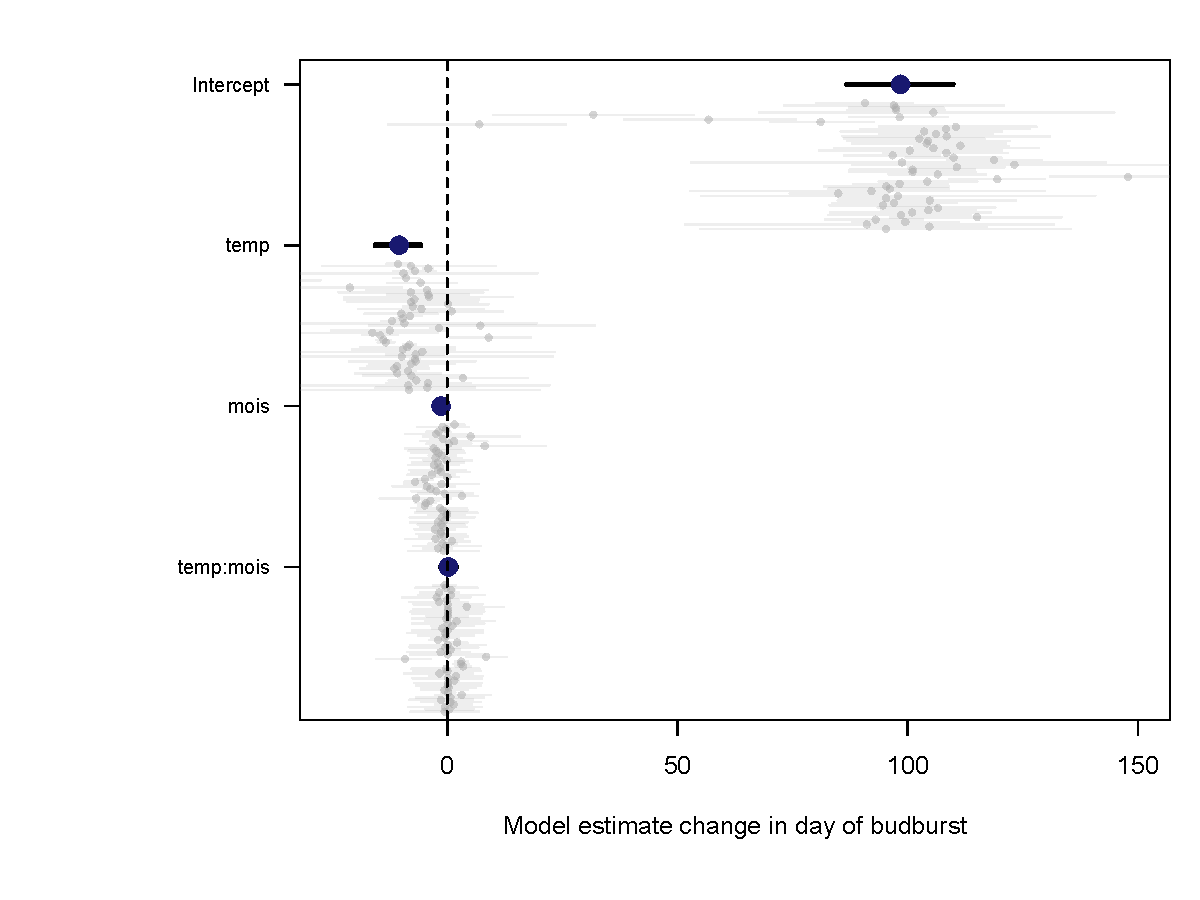
\includegraphics{/Users/aileneettinger/git/radcliffe/Analyses/soilmoisture/figures/m5bbd.pdf}
 \caption{\textbf{Model coefficients from budburst model (with centered predictors).}} 
 \label{fig:bb}
 \end{figure}

%\begin{figure}[h]
%\centering
% 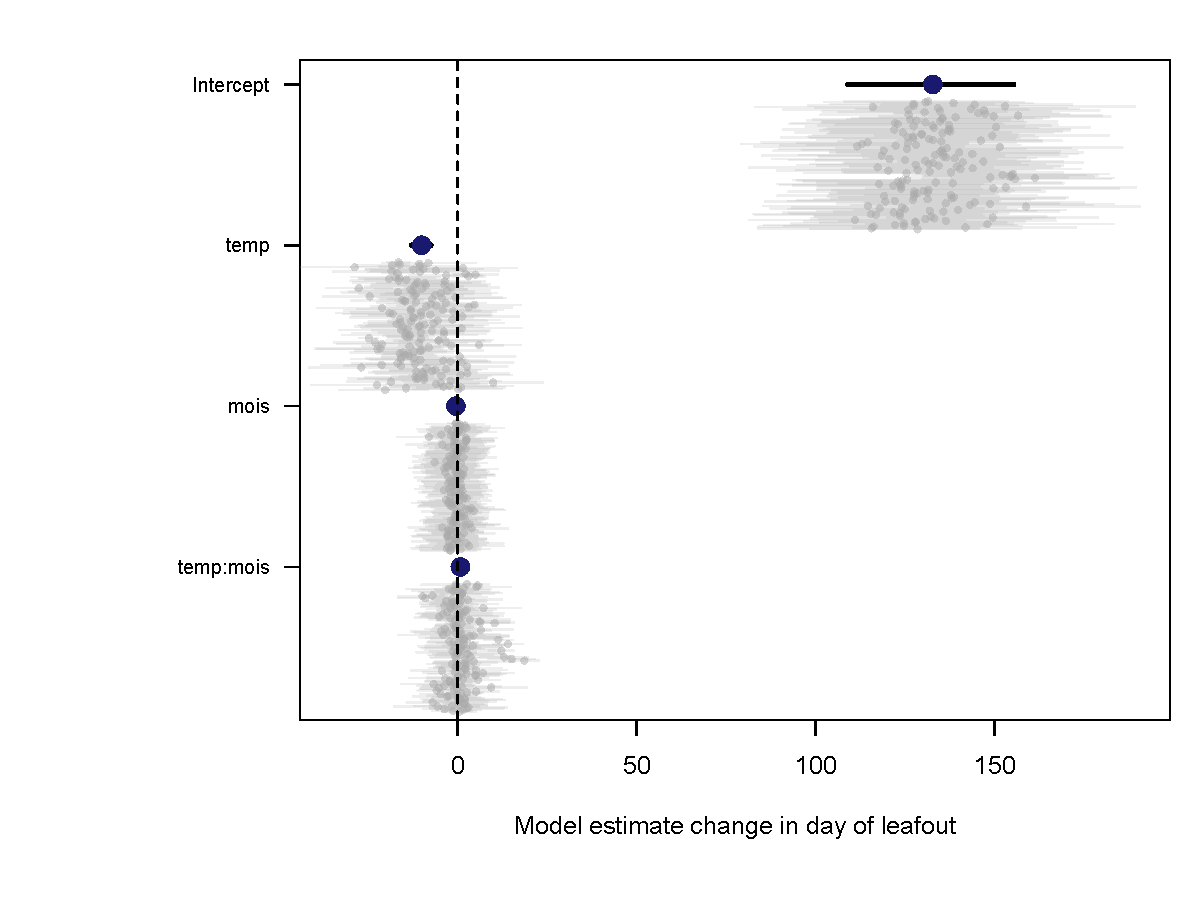
\includegraphics{/Users/aileneettinger/git/radcliffe/Analyses/soilmoisture/figures/m5lod.pdf}
% \caption{\textbf{Model coefficients from leafout model (with centered predictors).}} 
% \label{fig:lo}
% \end{figure}

%\begin{figure}[h]
%\centering
% 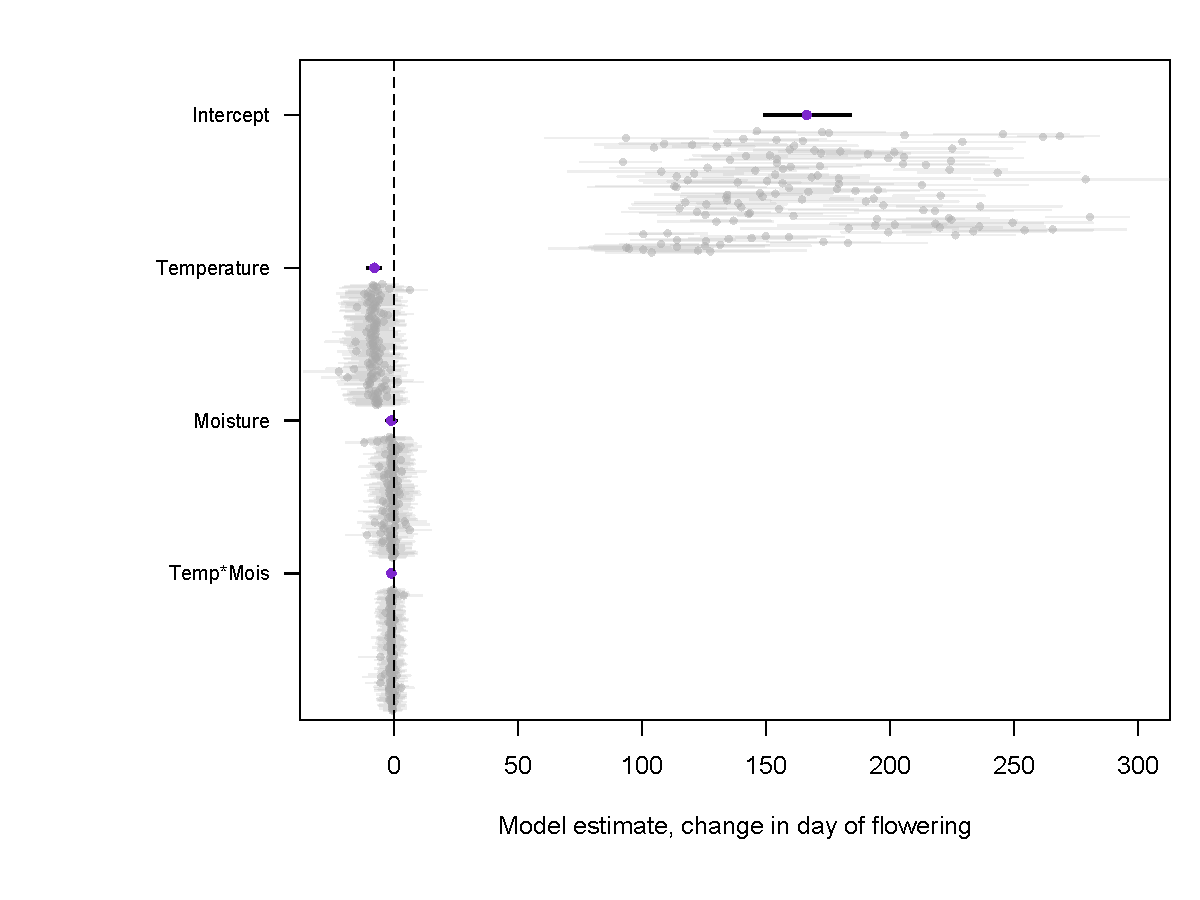
\includegraphics{/Users/aileneettinger/git/radcliffe/Analyses/soilmoisture/figures/m5ffd.pdf}
% \caption{\textbf{Model coefficients from first flower model (with centered predictors).}} 
% \label{fig:ff}
 %\end{figure}

%%%%%%%%%%%%%%%%%%%%%%%%%%%%%%%%%%%%%%%%
\end{document}
%%%%%%%%%%%%%%%%%%%%%%%%%%%%%%%%%%%%%%%%
